\section{Spark::Sp\-Maths$<$ Real $>$ Class Template Reference}
\label{classSpark_1_1SpMaths}\index{Spark::SpMaths@{Spark::SpMaths}}
{\tt \#include $<$Sp\-Maths.h$>$}

Collaboration diagram for Spark::Sp\-Maths$<$ Real $>$:\begin{figure}[H]
\begin{center}
\leavevmode
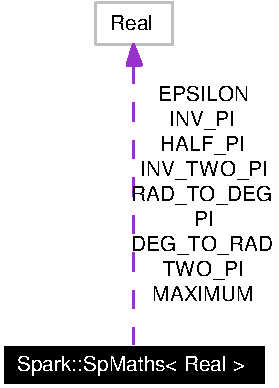
\includegraphics[width=84pt]{classSpark_1_1SpMaths__coll__graph}
\end{center}
\end{figure}


\subsection{Detailed Description}
\subsubsection*{template$<$class Real$>$ class Spark::Sp\-Maths$<$ Real $>$}

Static utility class for mathematical constants. 

Definition at line 37 of file Sp\-Maths.h.\subsection*{Static Public Attributes}
\begin{CompactItemize}
\item 
const Real {\bf PI} = (float)(4.0$\ast$atan(1.0))
\begin{CompactList}\small\item\em Static Constants:. \item\end{CompactList}\item 
const Real {\bf TWO\_\-PI} = 2.0f$\ast${\bf Sp\-Maths}$<$float$>$::{\bf PI}
\item 
const Real {\bf HALF\_\-PI} = 0.5f$\ast${\bf Sp\-Maths}$<$float$>$::{\bf PI}
\item 
const Real {\bf INV\_\-PI} = 1.0f/{\bf Sp\-Maths}$<$float$>$::{\bf PI}
\item 
const Real {\bf INV\_\-TWO\_\-PI} = 1.0f/{\bf Sp\-Maths}$<$float$>$::{\bf TWO\_\-PI}
\item 
const Real {\bf DEG\_\-TO\_\-RAD} = {\bf Sp\-Maths}$<$float$>$::{\bf PI}/180.0f
\item 
const Real {\bf RAD\_\-TO\_\-DEG} = 180.0f/{\bf Sp\-Maths}$<$float$>$::{\bf PI}
\item 
const Real {\bf EPSILON} = FLT\_\-EPSILON
\item 
const Real {\bf MAXIMUM} = FLT\_\-MAX
\end{CompactItemize}


\subsection{Member Data Documentation}
\index{Spark::SpMaths@{Spark::Sp\-Maths}!DEG_TO_RAD@{DEG\_\-TO\_\-RAD}}
\index{DEG_TO_RAD@{DEG\_\-TO\_\-RAD}!Spark::SpMaths@{Spark::Sp\-Maths}}
\subsubsection{\setlength{\rightskip}{0pt plus 5cm}template$<$class Real$>$ const double {\bf Spark::Sp\-Maths}$<$$>$::{\bf DEG\_\-TO\_\-RAD} = {\bf Sp\-Maths}$<$float$>$::{\bf PI}/180.0f\hspace{0.3cm}{\tt  [static]}}\label{classSpark_1_1SpMaths_s5}


Definition at line 30 of file Sp\-Maths.cpp.\index{Spark::SpMaths@{Spark::Sp\-Maths}!EPSILON@{EPSILON}}
\index{EPSILON@{EPSILON}!Spark::SpMaths@{Spark::Sp\-Maths}}
\subsubsection{\setlength{\rightskip}{0pt plus 5cm}template$<$class Real$>$ const double {\bf Spark::Sp\-Maths}$<$$>$::{\bf EPSILON} = FLT\_\-EPSILON\hspace{0.3cm}{\tt  [static]}}\label{classSpark_1_1SpMaths_s7}


Definition at line 23 of file Sp\-Maths.cpp.\index{Spark::SpMaths@{Spark::Sp\-Maths}!HALF_PI@{HALF\_\-PI}}
\index{HALF_PI@{HALF\_\-PI}!Spark::SpMaths@{Spark::Sp\-Maths}}
\subsubsection{\setlength{\rightskip}{0pt plus 5cm}template$<$class Real$>$ const double {\bf Spark::Sp\-Maths}$<$$>$::{\bf HALF\_\-PI} = 0.5f$\ast${\bf Sp\-Maths}$<$float$>$::{\bf PI}\hspace{0.3cm}{\tt  [static]}}\label{classSpark_1_1SpMaths_s2}


Definition at line 27 of file Sp\-Maths.cpp.\index{Spark::SpMaths@{Spark::Sp\-Maths}!INV_PI@{INV\_\-PI}}
\index{INV_PI@{INV\_\-PI}!Spark::SpMaths@{Spark::Sp\-Maths}}
\subsubsection{\setlength{\rightskip}{0pt plus 5cm}template$<$class Real$>$ const double {\bf Spark::Sp\-Maths}$<$$>$::{\bf INV\_\-PI} = 1.0f/{\bf Sp\-Maths}$<$float$>$::{\bf PI}\hspace{0.3cm}{\tt  [static]}}\label{classSpark_1_1SpMaths_s3}


Definition at line 28 of file Sp\-Maths.cpp.\index{Spark::SpMaths@{Spark::Sp\-Maths}!INV_TWO_PI@{INV\_\-TWO\_\-PI}}
\index{INV_TWO_PI@{INV\_\-TWO\_\-PI}!Spark::SpMaths@{Spark::Sp\-Maths}}
\subsubsection{\setlength{\rightskip}{0pt plus 5cm}template$<$class Real$>$ const double {\bf Spark::Sp\-Maths}$<$$>$::{\bf INV\_\-TWO\_\-PI} = 1.0f/{\bf Sp\-Maths}$<$float$>$::{\bf TWO\_\-PI}\hspace{0.3cm}{\tt  [static]}}\label{classSpark_1_1SpMaths_s4}


Definition at line 29 of file Sp\-Maths.cpp.\index{Spark::SpMaths@{Spark::Sp\-Maths}!MAXIMUM@{MAXIMUM}}
\index{MAXIMUM@{MAXIMUM}!Spark::SpMaths@{Spark::Sp\-Maths}}
\subsubsection{\setlength{\rightskip}{0pt plus 5cm}template$<$class Real$>$ const double {\bf Spark::Sp\-Maths}$<$$>$::{\bf MAXIMUM} = FLT\_\-MAX\hspace{0.3cm}{\tt  [static]}}\label{classSpark_1_1SpMaths_s8}


Definition at line 24 of file Sp\-Maths.cpp.\index{Spark::SpMaths@{Spark::Sp\-Maths}!PI@{PI}}
\index{PI@{PI}!Spark::SpMaths@{Spark::Sp\-Maths}}
\subsubsection{\setlength{\rightskip}{0pt plus 5cm}template$<$class Real$>$ const double {\bf Spark::Sp\-Maths}$<$$>$::{\bf PI} = (float)(4.0$\ast$atan(1.0))\hspace{0.3cm}{\tt  [static]}}\label{classSpark_1_1SpMaths_s0}


Static Constants:. 

Definition at line 25 of file Sp\-Maths.cpp.\index{Spark::SpMaths@{Spark::Sp\-Maths}!RAD_TO_DEG@{RAD\_\-TO\_\-DEG}}
\index{RAD_TO_DEG@{RAD\_\-TO\_\-DEG}!Spark::SpMaths@{Spark::Sp\-Maths}}
\subsubsection{\setlength{\rightskip}{0pt plus 5cm}template$<$class Real$>$ const double {\bf Spark::Sp\-Maths}$<$$>$::{\bf RAD\_\-TO\_\-DEG} = 180.0f/{\bf Sp\-Maths}$<$float$>$::{\bf PI}\hspace{0.3cm}{\tt  [static]}}\label{classSpark_1_1SpMaths_s6}


Definition at line 31 of file Sp\-Maths.cpp.\index{Spark::SpMaths@{Spark::Sp\-Maths}!TWO_PI@{TWO\_\-PI}}
\index{TWO_PI@{TWO\_\-PI}!Spark::SpMaths@{Spark::Sp\-Maths}}
\subsubsection{\setlength{\rightskip}{0pt plus 5cm}template$<$class Real$>$ const double {\bf Spark::Sp\-Maths}$<$$>$::{\bf TWO\_\-PI} = 2.0f$\ast${\bf Sp\-Maths}$<$float$>$::{\bf PI}\hspace{0.3cm}{\tt  [static]}}\label{classSpark_1_1SpMaths_s1}


Definition at line 26 of file Sp\-Maths.cpp.

The documentation for this class was generated from the following files:\begin{CompactItemize}
\item 
{\bf Sp\-Maths.h}\item 
{\bf Sp\-Maths.cpp}\end{CompactItemize}
